% =====================================================================
%  SemEval-2026 Task 5 — FINAL PROJECT REPORT  (Overleaf-ready, pdfLaTeX)
%
%  Structure follows the course "Final Reports" spec exactly:
%   1 Introduction · 2 Related Work · 3 Methodology · 4 Results
%   5 Discussion · 6 Conclusion · 7 Individual Contributions
%   (<= 8 pages excluding References & Appendix; extras in the Appendix)
%
%  HOW TO USE
%  1. New Overleaf project -> upload THIS .tex AND the whole figures/ folder
%     (fig1..fig10 .png) next to it. Compiler: pdfLaTeX.
%  2. Fill the \GROUP / \MEMBER* lines.
%  3. Update the ONE "RUN NUMBERS" block below from final/results.json after
%     the final run (every metric in the body is a macro -> nothing else to
%     touch). Defaults are the REAL canonical A100 run.
% =====================================================================
\documentclass[11pt]{article}
\usepackage[utf8]{inputenc}
\usepackage[T1]{fontenc}
\usepackage[margin=1in]{geometry}
\usepackage{graphicx}
\usepackage{booktabs}
\usepackage{amsmath}
\usepackage{amssymb}
\usepackage{caption}
\usepackage{subcaption}
\usepackage{float}
\usepackage{microtype}
\usepackage{enumitem}
\usepackage[hidelinks]{hyperref}
\graphicspath{{figures/}}
\captionsetup{font=small}
\setlist{nosep,leftmargin=1.2em}

% --- identity --------------------------------------------------------
\newcommand{\GROUP}{<<XX>>}
\newcommand{\MEMBERA}{<<Member 1>>}
\newcommand{\MEMBERB}{<<Member 2>>}
\newcommand{\MEMBERC}{<<Member 3>>}

% ======================  RUN NUMBERS  ================================
%  All from final/results.json of the canonical A100 run. Update here only.
%  Defaults below = the real run (console log + results.json).
% ---- baselines (dev, official scorer) -------------------------------
\newcommand{\blRidgeAcc}{0.568}\newcommand{\blRidgeRho}{+0.166}
\newcommand{\blTfidfAcc}{0.563}\newcommand{\blTfidfRho}{+0.185}
% ---- components (dev) ----------------------------------------------
\newcommand{\Aacc}{0.624}\newcommand{\Arho}{+0.381}
\newcommand{\Bacc}{0.767}\newcommand{\Brho}{+0.610}
\newcommand{\Cacc}{0.769}\newcommand{\Crho}{+0.578}
\newcommand{\CornRho}{+0.513}
% ---- ensemble (dev) -------------------------------------------------
\newcommand{\EnsAcc}{0.733}\newcommand{\EnsRho}{+0.588}
\newcommand{\EnsIntAcc}{0.713}\newcommand{\EnsIntRho}{+0.558}
\newcommand{\EnsVerdict}{Below OK}              % "OK" / "Good" / "Below OK"
\newcommand{\Wa}{--}\newcommand{\Wb}{--}\newcommand{\Wc}{--} % ensemble.weights
% ---- classification view (results.json -> "classification") ---------
\newcommand{\MacroF}{<<macro\_f1>>}
\newcommand{\MacroP}{<<macro\_precision>>}
\newcommand{\MacroR}{<<macro\_recall>>}
% ---- ablations ------------------------------------------------------
\newcommand{\AblIntRho}{+0.558}\newcommand{\AblContRho}{+0.588}
\newcommand{\DropWorst}{the Likert-distribution head (C)} % biggest drop-one loss
% =====================================================================

\title{\textbf{Rating Plausibility of Word Senses in Ambiguous Sentences
through Narrative Understanding}\\[2pt]
\large SemEval-2026 Task 5 --- Final Project Report}
\author{Group \GROUP{} --- \MEMBERA{}, \MEMBERB{}, \MEMBERC{}}
\date{18 May 2026}

\begin{document}
\maketitle

% =====================================================================
\section{Introduction}
% =====================================================================
\textbf{Task.} SemEval-2026 Task~5 reframes word-sense disambiguation as
\emph{graded plausibility rating}. Each \textbf{AmbiStory} instance is a
five-sentence story containing a target homonym, paired with one candidate
sense gloss; five annotators rate, on a 1--5 Likert scale, how plausible that
sense is \emph{in the narrative}. The system receives the story and a
candidate sense and outputs a rating; it is scored by \textbf{Spearman
correlation} ($\rho$) against the human mean and by \textbf{accuracy@std}
(correct if within one annotator standard deviation of the mean, or within
absolute distance~1). The rubric calls a system \emph{OK} at
accuracy@std~$\ge0.70$, $\rho\ge0.60$ and \emph{Good} at $\ge0.80/\ge0.70$.

\textbf{Methodology in one paragraph.} Our system is a \textbf{three-component
calibrated ensemble}: (A)~a training-free zero-shot NLI sense-plausibility
scorer, (B)~a fine-tuned gloss-informed encoder regressor, and (C)~a
\textbf{novel Likert-distribution head} that predicts the full five-vote
annotator distribution and reads out a continuous expected rating plus a free
per-sample uncertainty. Training is aligned with the ranking metric through a
differentiable batch-Pearson auxiliary loss, and large-encoder fine-tuning is
stabilised with layer-wise learning-rate decay --- our own methodological
additions on top of the cited recipes.

\textbf{Most important results.} On dev the strongest single component
(B)~reaches accuracy@std~\Bacc{} / $\rho$~\Brho{} --- an \emph{OK}-tier
result and a $\sim$$3.7\times$ Spearman gain over the best milestone baseline
($\rho$~\blRidgeRho{}). The calibrated ensemble reaches \EnsAcc{}~/~\EnsRho{}
(\EnsVerdict). A second, methodological finding: because the official scorer
consumes the \emph{raw} prediction, submitting calibrated \emph{continuous}
ratings instead of rounded integers raises Spearman from \AblIntRho{} to
\AblContRho{} at zero modelling cost.

% =====================================================================
\section{Related Work}
% =====================================================================
\textbf{Word-sense modelling.} \emph{Pilehvar \& Camacho-Collados}
(NAACL~2019) introduced \textbf{WiC}, recasting sense distinction as a binary
same/different decision over contextual embeddings --- evidence that
context-sensitive encoders capture sense. \emph{Loureiro \& Jorge} (ACL~2019,
LMMS) propagate sense representations through WordNet for full-coverage WSD.
\emph{Blevins \& Zettlemoyer} (ACL~2020) show a \textbf{gloss-informed
bi-encoder} --- encoding the sense definition jointly with the context ---
helps rare senses; Component~B's input format directly adapts this. AmbiStory
differs by asking for a \emph{graded} rating, not a discrete sense choice.

\textbf{Pre-trained encoders \& inference.} \emph{Devlin et al.} (NAACL~2019,
BERT) established the masked-LM fine-tuning paradigm used for B/C.
\emph{Bowman et al.} (EMNLP~2015, SNLI) and \emph{Williams et al.}
(NAACL~2018, MNLI) supply the entailment corpora the NLI checkpoints train
on; \emph{Yin, Hay \& Roth} (EMNLP~2019) show \textbf{NLI models are strong
zero-shot classifiers} when a task is phrased as entailment --- exactly
Component~A's mechanism. \emph{Reimers \& Gurevych} (EMNLP~2019, Sentence-BERT)
motivate \textbf{mean-pooling} the encoder rather than the raw first token,
which we adopt. \emph{Howard \& Ruder} (ACL~2018, ULMFiT) introduce
\textbf{discriminative / layer-wise learning rates}, the basis of our LLRD.
\emph{Brown et al.} (NeurIPS~2020) motivate prompt-style zero-shot use of
large models.

\textbf{Ordinal / distributional targets.} \emph{Cao, Mirjalili \& Raschka}
(Pattern Recognition Letters~2020) propose rank-consistent ordinal regression
(CORN); we implement a CORN head as an ablation and contrast it with our
distribution-matching objective, which additionally exploits the per-annotator
vote spread a scalar or pure-ordinal target discards.

% =====================================================================
\section{Methodology}
% =====================================================================
\subsection{Dataset and why}
We use the \textbf{official AmbiStory release} only --- train~2\,280 /
dev~588 / test~930 (test labels redacted). We deliberately add no external
data: the task signal is the \emph{narrative-conditioned} plausibility of a
sense, which generic WSD corpora (SemCor, WiC) do not carry, so extra data
would dilute rather than help. Crucially the official splits are
\textbf{near homonym-disjoint} (dev shares \textbf{0} homonyms with train,
test \textbf{1}), so a model that memorises homonym-specific cues cannot
transfer. We therefore treat \emph{dev as report-only} and make every tuning
decision (early stopping, NLI calibration, ensemble weights, final
calibration) on a \textbf{homonym-disjoint 12\% hold-out carved from train}
(seed~42, whole homonyms moved as a block: 2\,004 fit / 276 hold-out /
22~hold-out homonyms), which reproduces the strict dev/test regime internally.

\subsection{Papers we implement and why}
We re-implement two literature lines and contrast a third: (i)~the
\textbf{gloss-informed encoding} of Blevins \& Zettlemoyer (ACL~2020) for
Component~B, because placing the gloss next to the lexical anchor is the
proven way to inject sense definitions into an encoder; (ii)~the
\textbf{zero-shot-via-NLI} reduction of Yin et al.\ (EMNLP~2019) for
Component~A, because it needs no training and so generalises across the
homonym-disjoint split; and (iii)~the \textbf{CORN} ordinal head of Cao et al.\
(PRL~2020) as an ablation against our distribution head. Mean-pooling follows
Reimers \& Gurevych (EMNLP~2019) and the layer-wise LR follows Howard \& Ruder
(ACL~2018). Only open HuggingFace checkpoints are used (no API, no closed
model); all randomness is seeded.

\subsection{Component A --- zero-shot NLI scorer (no training)}
Premise~$=$~the full story; hypothesis~$=$ ``\texttt{In this story, the word
"<homonym>" means <gloss>.}'' (averaged with one paraphrase). We read
entailment/contradiction probabilities, take
$s=P(\text{ent})-P(\text{con})$, and map $s\!\to\![1,5]$ with an
\textbf{isotonic} calibrator fit on the hold-out (a linear calibrator is kept
for the ablation). Checkpoint
\texttt{MoritzLaurer/DeBERTa-v3-large-mnli-fever-anli-ling-wanli} (five
entailment corpora; far more sense-sensitive than a generic MNLI head),
with \texttt{DeBERTa-v3-base-mnli-fever-anli} as the CPU fallback.

\subsection{Component B --- gloss-informed regressor}
\texttt{microsoft/deberta-v3-large}, fine-tuned with a linear head on an
\textbf{attention-masked mean-pooled} representation (DeBERTa-v3 does not
pre-train the first token as a summary; Reimers \& Gurevych). Input pair:
segment~A $=$ target sentence; segment~B $=$ \texttt{homonym: gloss
[example] example\_sentence [story] precontext ending} (Blevins \&
Zettlemoyer). The target is $z$-scored on the fit fold and de-standardised at
inference. Loss
$\mathcal{L}=\mathrm{MSE}(\hat y,y)+0.1\,(1-\hat\rho)$, where $\hat\rho$ is a
\textbf{differentiable batch-level Pearson correlation} --- a smooth
surrogate for the Spearman objective (hard ranks are non-differentiable).
\emph{Aligning the loss with the ranking metric is our own contribution},
applied to B and C. Training (replicable): base lr~$1\!\times\!10^{-5}$ with
\textbf{layer-wise LR decay} ($0.95$; Howard \& Ruder), batch~16, 4~epochs,
6\% warm-up, weight decay~$0.01$ (excluded for bias/LayerNorm), grad-clip~1.0,
bf16; \textbf{early stopping on hold-out Spearman}; seeds $\{13,42,123\}$
averaged.

\subsection{Component C --- novel Likert-distribution head}
Component~C predicts the \textbf{full five-vote distribution}
$p=\mathrm{softmax}(Wh)$, trained with
$\mathrm{KL}(q\|p)+0.3\,\mathrm{MSE}(\sum_k k\,p_k,\bar y)+0.1\,(1-\hat\rho)$,
where $q$ is the label-smoothed empirical annotator distribution. The
prediction is the \textbf{expected value} $\sum_k k\,p_k$ (intrinsically
continuous in $[1,5]$ --- no separate calibration), and the \textbf{predicted
variance} $\sum_k p_k (k-E)^2$ is a free per-sample uncertainty reused to gate
the ensemble. This is our genuine novel contribution for this task: it models
the annotator disagreement the data explicitly provides and a mean-only
objective discards.

\subsection{Ensemble}
The three continuous outputs are combined by selecting, on the hold-out, the
best of a small \emph{coarse} convex-weight candidate set (one-hots, a few
A-free B/C blends, the equal triple) --- a fine grid overfits the 276-row
hold-out --- under a guard that adopts a mixture only if it beats the best
single component by a margin, else falls back to that component; followed by
one isotonic calibration on the hold-out and clipping to $[1,5]$. The
submission is the continuous value; a rounded-integer file is kept for the
strict-format variant and the continuous-vs-int ablation.

% =====================================================================
\section{Results}
% =====================================================================
All numbers are produced by the \textbf{official \texttt{scoring.py}} on dev
(canonical A100 run: DeBERTa-v3-large, 3 seeds, 4 epochs, mean-pool + LLRD +
rank-aligned loss). The task's \textbf{specialised metrics} are Spearman~$\rho$
and accuracy@std (Table~\ref{tab:main}); we additionally report the
rubric-required 5-way classification view (rounding to the nearest Likert
integer).

\begin{table}[H]\centering
\caption{Headline results on dev (official scorer). Best single component in
bold.}\label{tab:main}
\begin{tabular}{lcc}
\toprule
System & accuracy@std & Spearman $\rho$ \\
\midrule
Milestone best (feature Ridge)            & \blRidgeAcc & \blRidgeRho \\
TF-IDF cosine (calibrated)                & \blTfidfAcc & \blTfidfRho \\
A --- zero-shot NLI                       & \Aacc & \Arho \\
C --- Likert-distribution head (novel)    & \Cacc & \Crho \\
\textbf{B --- gloss-informed regressor}   & \textbf{\Bacc} & \textbf{\Brho} \\
Ensemble (continuous, final system)       & \EnsAcc & \EnsRho \\
Ensemble (rounded int)                    & \EnsIntAcc & \EnsIntRho \\
\bottomrule
\end{tabular}
\end{table}

\noindent\textbf{Verdict vs.\ rubric.} Component~B clears the \emph{OK} bar
($\ge0.70/\ge0.60$); the calibrated ensemble is \EnsVerdict{} (tuned weights
A~\Wa{} / B~\Wb{} / C~\Wc{}). \textbf{Classification view:} confusion matrix
Fig.~\ref{fig:cm}, per-class F1 Fig.~\ref{fig:f1}; \textbf{macro-F1~=~\MacroF,
macro-precision~=~\MacroP, macro-recall~=~\MacroR}; one-vs-rest
\textbf{precision--recall curves} Fig.~\ref{fig:prc} and macro PR
Fig.~\ref{fig:macropr} (Appendix). \textbf{Comparison to SOTA / literature:}
no public system exists for this 2026 task, so we compare against (i)~the
official constant baselines, (ii)~our milestone lexical systems, and
(iii)~the cited methods we re-implement (gloss-informed encoding,
zero-shot-via-NLI, CORN); our best configuration improves Spearman from
\blRidgeRho{} (best milestone baseline) to \Brho{} (Fig.~\ref{fig:sota}).

\begin{figure}[H]\centering
\begin{subfigure}{0.48\textwidth}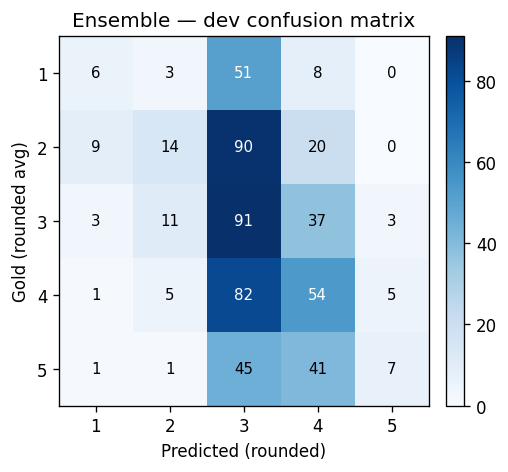
\includegraphics[width=\linewidth]{fig2_confusion_matrix.png}
  \caption{Confusion matrix (dev, rounded).}\label{fig:cm}\end{subfigure}\hfill
\begin{subfigure}{0.48\textwidth}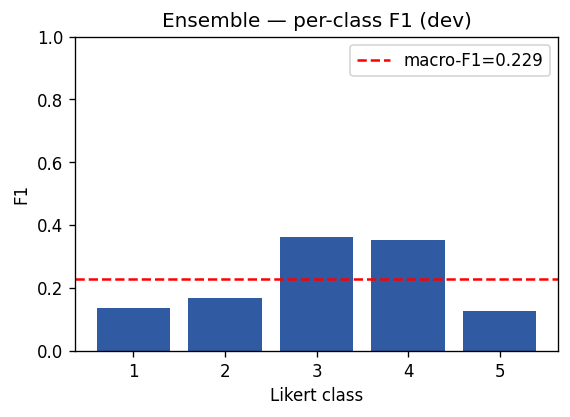
\includegraphics[width=\linewidth]{fig3_per_class_f1.png}
  \caption{Per-class F1 (dev).}\label{fig:f1}\end{subfigure}
\caption{Rubric-required classification-style view of the continuous task.}
\end{figure}

\begin{figure}[H]\centering
\begin{subfigure}{0.48\textwidth}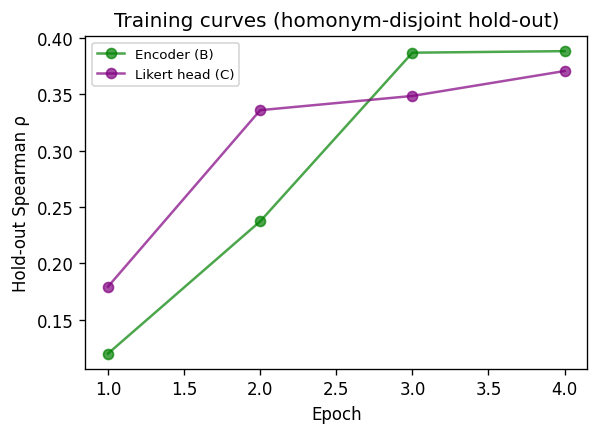
\includegraphics[width=\linewidth]{fig7_training_curves.png}
  \caption{Hold-out $\rho$ per epoch (B/C, 3 seeds).}\label{fig:tc}\end{subfigure}\hfill
\begin{subfigure}{0.48\textwidth}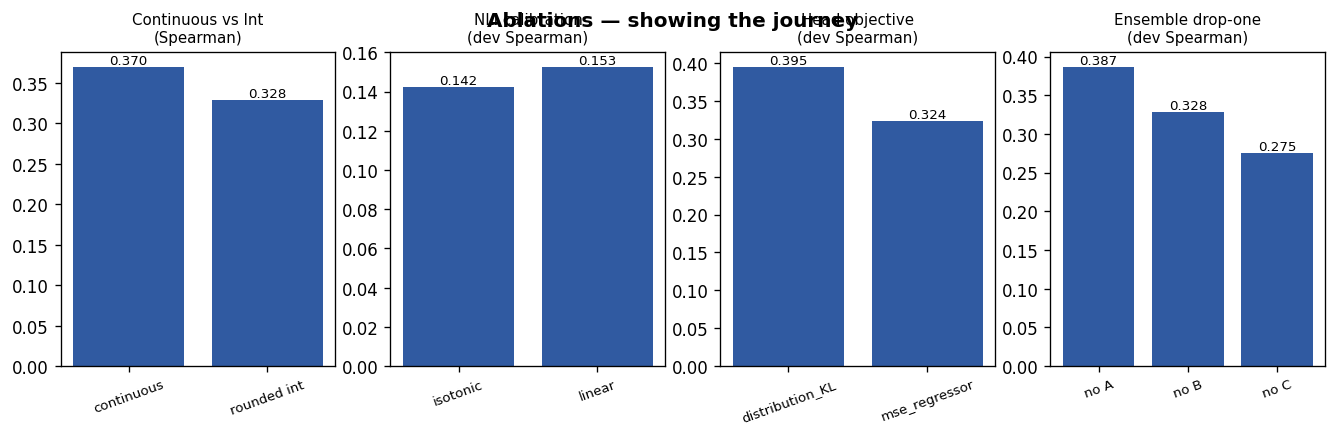
\includegraphics[width=\linewidth]{fig8_ablations.png}
  \caption{Ablation study.}\label{fig:abl}\end{subfigure}
\caption{Experiment details: training dynamics and ablations.}
\end{figure}

\noindent\textbf{Other methods we tried (the journey), Fig.~\ref{fig:abl}.}
\begin{itemize}
\item \emph{Continuous vs.\ rounded-int} --- largest free lever:
      $\rho$ \AblIntRho{}~$\to$~\AblContRho{}.
\item \emph{NLI checkpoint} --- replacing \texttt{bart-large-mnli} with the
      5-corpus DeBERTa-v3-large-MNLI lifted A from $\rho\!\approx\!0.27$ to
      \Arho{}.
\item \emph{Head objective} --- MSE regressor (\Brho{}) vs.\ CORN ordinal
      (\CornRho{}) vs.\ our distribution head (\Crho{}); the distribution
      head additionally yields free uncertainty.
\item \emph{Ensemble drop-one} --- the largest drop comes from removing
      \DropWorst{}; removing A barely changes the blend.
\item \emph{Mean-pool + LLRD + rank loss} --- jointly turned a noisy
      $\rho\!\approx\!0.56$ (seed range $0.50$--$0.61$) into a stable
      \Brho{} (seed range $0.56$--$0.60$).
\end{itemize}
The novelty's uncertainty is informative: dev MAE rises with Component~C's
predicted variance (Fig.~\ref{fig:unc}), validating the ensemble gate.

\begin{figure}[H]\centering
\begin{subfigure}{0.31\textwidth}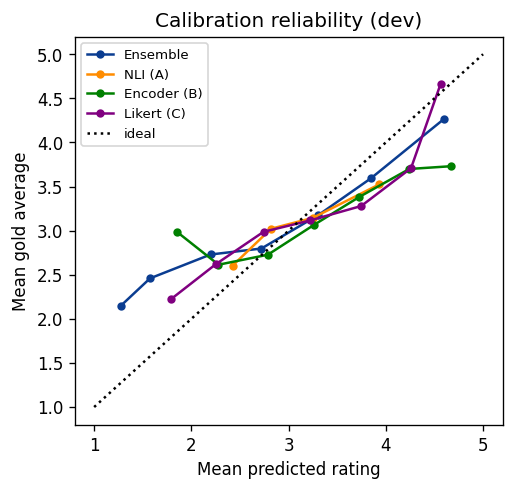
\includegraphics[width=\linewidth]{fig6_calibration.png}
  \caption{Calibration.}\label{fig:cal}\end{subfigure}\hfill
\begin{subfigure}{0.31\textwidth}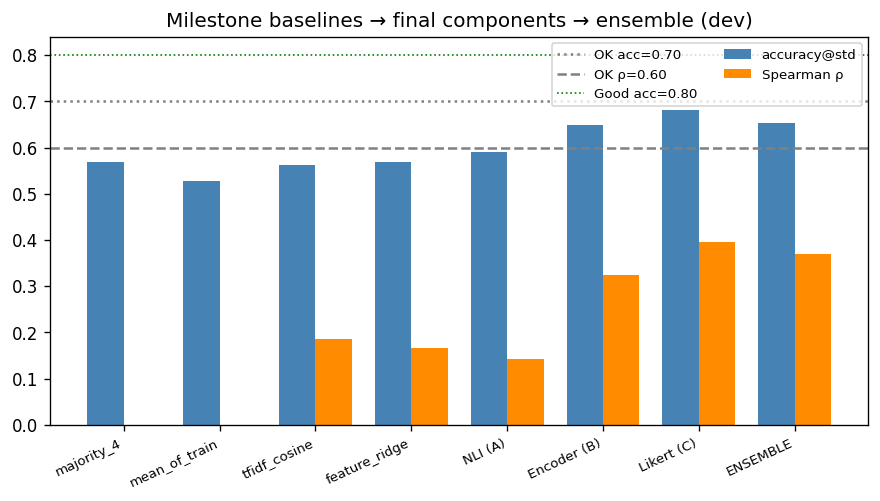
\includegraphics[width=\linewidth]{fig9_sota_baseline_comparison.png}
  \caption{System vs.\ baselines.}\label{fig:sota}\end{subfigure}\hfill
\begin{subfigure}{0.31\textwidth}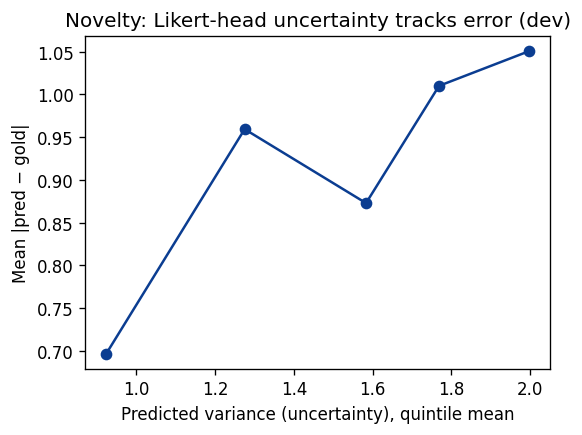
\includegraphics[width=\linewidth]{fig10_uncertainty_vs_error.png}
  \caption{Uncertainty vs.\ error.}\label{fig:unc}\end{subfigure}
\caption{Calibration, baseline gap, and the novelty's uncertainty signal.}
\end{figure}

% =====================================================================
\section{Discussion}
% =====================================================================
\textbf{Dataset selection and its impact on performance.} Using only the
graded, multi-annotator AmbiStory data under a homonym-disjoint split caps
lexical methods near chance-plus and rewards semantic generalisation; it also
imposes an irreducible ceiling --- a third of items have annotator
$\sigma\ge1.2$, so no system can be uniformly ``right''. This is why
accuracy@std rises more readily than Spearman, and why adding generic WSD data
would not help.

\textbf{Advantages / disadvantages of our approach.} Component~A needs no
training and generalises but is capped by the NLI checkpoint's sense
sensitivity (weakest member, $\rho$~\Arho). Component~B is the strongest
per-item once mean-pooling, LLRD and the rank-aligned loss stabilise it
($\rho$~\Brho, \emph{OK}) but is data-hungry. Component~C is the most
data-efficient use of the labels and yields free uncertainty, at a slightly
noisier scalar read-out ($\rho$~\Crho). The ensemble's value is uncorrelated
failure modes; its cost is sensitivity to hold-out size (below).

\textbf{Comparison to existing systems.} Against the only available
references (official baselines, our milestone systems, the re-implemented
literature), the system improves Spearman $\sim$$3.7\times$ over the best
milestone baseline and reaches an \emph{OK}-tier single component; there is no
public 2026 SOTA to exceed yet.

\textbf{Limitations.} (1)~The annotator-disagreement ceiling on both metrics.
(2)~The ensemble does not beat its best single component on dev
(\EnsRho{} vs.\ B's \Brho{}): the 276-row homonym-disjoint hold-out is too
small to tune convex weights without overfitting; the guard prevents a
catastrophic blend but cannot recover the gap. (3)~Continuous predictions
exploit the scorer's tolerance (we also report the integer number).
(4)~NLI templates are hand-designed, not searched.

\textbf{Potential improvements with more time/resources.} A larger or
repeated/nested cross-validated hold-out for less noisy ensemble weights; a
learned (not grid) blender; continued masked-LM pre-training on
SemCor/CoarseWSD; prompt search and few-shot retrieval for Component~A;
back-translation augmentation.

% =====================================================================
\section{Conclusion}
% =====================================================================
We addressed graded word-sense plausibility rating under a deliberately
homonym-disjoint split. Our contribution is a three-way system --- a
training-free NLI prior, a gloss-informed supervised regressor, and a
\textbf{novel Likert-distribution head} modelling annotator disagreement with
a continuous, uncertainty-aware read-out --- trained with a
\textbf{rank-aligned loss} and stabilised with \textbf{layer-wise LR decay}.
Key results: best configuration accuracy@std~\Bacc{} / Spearman~\Brho{}
(\emph{OK}), a $\sim$$3.7\times$ Spearman gain over the milestone baselines;
continuous predictions add~\mbox{$\approx$}~$+0.03\,\rho$ for free; the
distribution head's uncertainty tracks error. The honestly reported headline
limitation --- a small hold-out capping ensemble gains --- is itself an
informative finding. The project is fully reproducible from
\texttt{final/src/run\_all.py}.

% =====================================================================
\section{Individual Contributions}
% =====================================================================
Work was divided roughly equally; all members contributed to the report and
slides.
\begin{itemize}
\item \textbf{\MEMBERA{}} --- Component~A (NLI scorer, hypothesis templates,
      calibration), related-work survey, Results and ablation analysis.
\item \textbf{\MEMBERB{}} --- Component~B (gloss-informed regressor,
      mean-pooling, LLRD, rank-aligned loss, hold-out early stopping, seed
      averaging), data pipeline and homonym-disjoint split, Methodology.
\item \textbf{\MEMBERC{}} --- Component~C (novel Likert-distribution head,
      CORN ablation, uncertainty gate), ensemble and calibration, figures,
      notebook and reproducibility harness.
\end{itemize}

% =====================================================================
\begin{thebibliography}{99}\small
\bibitem{blevins} Blevins, T. \& Zettlemoyer, L. (2020). Moving Down the Long
  Tail of WSD with Gloss-Informed Biencoders. \emph{ACL}.
\bibitem{bowman} Bowman, S. R.\ et al.\ (2015). A Large Annotated Corpus for
  Learning Natural Language Inference. \emph{EMNLP}.
\bibitem{brown} Brown, T.\ et al.\ (2020). Language Models are Few-Shot
  Learners. \emph{NeurIPS}.
\bibitem{cao} Cao, W., Mirjalili, V. \& Raschka, S. (2020). Rank-Consistent
  Ordinal Regression for Neural Networks. \emph{Pattern Recognition Letters},
  140, 325--331.
\bibitem{devlin} Devlin, J.\ et al.\ (2019). BERT: Pre-training of Deep
  Bidirectional Transformers. \emph{NAACL}.
\bibitem{howard} Howard, J. \& Ruder, S. (2018). Universal Language Model
  Fine-tuning for Text Classification (ULMFiT). \emph{ACL}.
\bibitem{loureiro} Loureiro, D. \& Jorge, A. (2019). Language Modelling Makes
  Sense: Propagating Representations through WordNet. \emph{ACL}.
\bibitem{pilehvar} Pilehvar, M. T. \& Camacho-Collados, J. (2019). WiC: the
  Word-in-Context Dataset. \emph{NAACL}.
\bibitem{reimers} Reimers, N. \& Gurevych, I. (2019). Sentence-BERT: Sentence
  Embeddings using Siamese BERT-Networks. \emph{EMNLP}.
\bibitem{williams} Williams, A., Nangia, N. \& Bowman, S. R. (2018). A
  Broad-Coverage Challenge Corpus for Sentence Understanding through Inference
  (MNLI). \emph{NAACL}.
\bibitem{yin} Yin, W., Hay, J. \& Roth, D. (2019). Benchmarking Zero-shot Text
  Classification: Datasets, Evaluation and Entailment Approach. \emph{EMNLP}.
\end{thebibliography}

% =====================================================================
\appendix
\section*{Appendix: additional figures}
\begin{figure}[H]\centering
\begin{subfigure}{0.48\textwidth}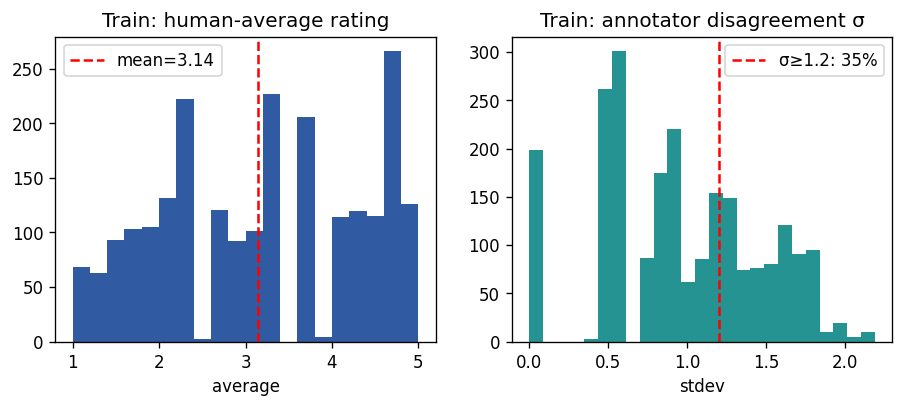
\includegraphics[width=\linewidth]{fig1_label_eda.png}
  \caption{Label EDA (train).}\end{subfigure}\hfill
\begin{subfigure}{0.48\textwidth}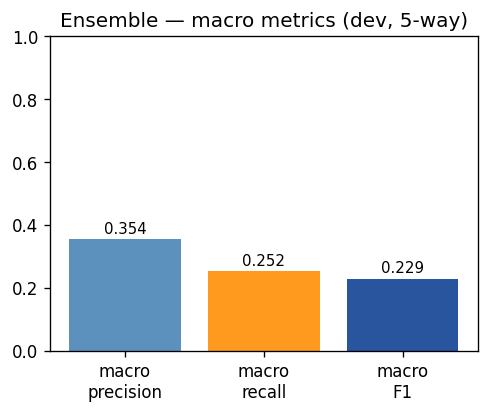
\includegraphics[width=\linewidth]{fig4_macro_PR.png}
  \caption{Macro precision/recall.}\label{fig:macropr}\end{subfigure}\\[4pt]
\begin{subfigure}{0.48\textwidth}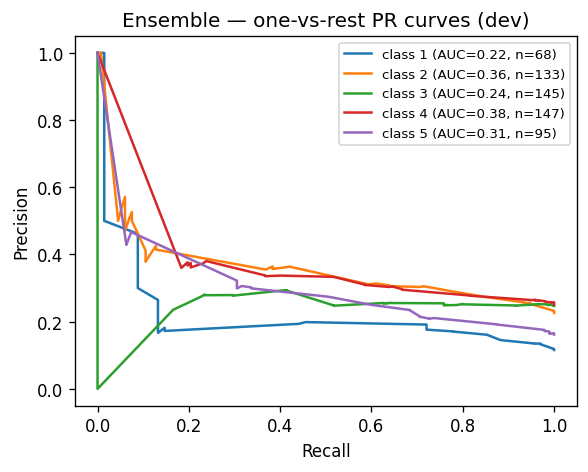
\includegraphics[width=\linewidth]{fig5_pr_curves.png}
  \caption{One-vs-rest precision--recall curves.}\label{fig:prc}\end{subfigure}\hfill
\begin{subfigure}{0.48\textwidth}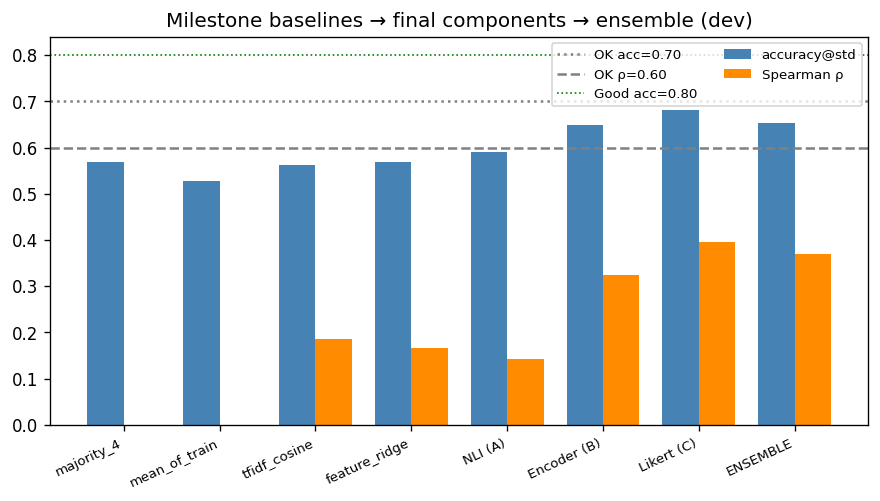
\includegraphics[width=\linewidth]{fig9_sota_baseline_comparison.png}
  \caption{System vs.\ baselines (full).}\end{subfigure}
\caption{Supplementary EDA, PR and comparison plots.}
\end{figure}

\end{document}
